\documentclass[color=usenames,dvipsnames]{beamer}

\usepackage{tikz}
\usepackage[utf8]{inputenc}

% smart quotes
\usepackage[autostyle, english=american]{csquotes}
\MakeOuterQuote{"}

% \usepackage{beamerthemesplit} // Activate for custom appearance

\title{Deep Neural Models\\for Bilingual Lexicon Extraction}
\author{Jon Gauthier and Arthur Tsang}
\date{28 May 2014}

\AtBeginSection[]
{
	\begin{frame}
		\tableofcontents[currentsection]
	\end{frame}
}

\begin{document}

\frame{\titlepage}

\section[Outline]{}
\frame{\tableofcontents}

\section{Introduction}
\subsection{Neural networks and translation}
\frame[label=howabout]
{
	\frametitle{How about this one?}
	\scalebox{2}{$f(\text{English}) = \text{Spanish}$}
}

\frame{
\resizebox{\linewidth}{!}{
\begin{tikzpicture}[font=\LARGE]
  \onslide<1->{
  \draw[rotate=15] (0, 0) rectangle (5, 8.09);
  \node (dog) [rotate=15] at (2, 6) {dog};
  \node (book) [rotate=15] at (1, 4) {book};
  \node (school) [rotate=15] at (2.4, 2.5) {school};

  \draw[rotate=-15] (6, 3) rectangle (11, 11.09);
  \node (perro) [rotate=-15] at (9.5, 6.5) {perro};
  \node (libro) [rotate=-15] at (10.5, 4.5) {libro};
  \node (escuela) [rotate=-15] at (9.25, 2.9) {escuela};
  }

  \onslide<2->{
  \draw[-latex] (dog) to[out=15, in=170, looseness=1]  (perro);
  \draw[-latex] (book) to[out=15, in=170, looseness=1]  (libro);
  \draw[-latex] (school) to[out=15, in=175, looseness=1]  (escuela);
  }
\end{tikzpicture}%
}
}

\section{The task: Bilingual lexicon extraction}

\frame{
\frametitle{Bilingual lexicon extraction}

Given multilingual corpora (composed of a \emph{source language} and \emph{target language}),\\~\\
\pause
learn \textbf{translation mappings} of the form
\pause

\[(\text{\emph{source language word}}, \text{\emph{target language word}})\]
}

\subsection{Standard lexical learning}

\frame{
\frametitle{\insertsubsectionhead}
\begin{figure}
\centering
\scalebox{2}{
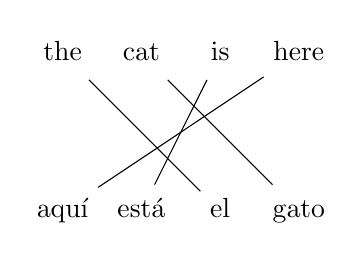
\begin{tikzpicture}
  \node (the) at (0, 2) {\strut the};
  \node (cat) at (1, 2) {\strut cat};
  \node (is) at (2, 2) {\strut is};
  \node (here) at (3, 2) {\strut here};

  \node (aqui) at (0, 0) {\strut aquí};
  \node (esta) at (1, 0) {\strut está};
  \node (el) at (2, 0) {\strut el};
  \node (gato) at (3, 0) {\strut gato};

  \onslide<2->{
  \draw (the) -- (el);
  \draw (cat) -- (gato);
  \draw (is) -- (esta);
  \draw (here) -- (aqui);
  }
\end{tikzpicture}
}
\end{figure}
}

\frame{
\frametitle{But we need parallel corpora for this..}
\begin{columns}
	\begin{column}{0.5\textwidth}
		{\color{Green} Soy siervo del Fuego Secreto, administrador de la llama de Anor.}
		{\color{Peach} ¡Tu fuego oscuro es en vano, llama de Udûn!}
		{\color{Sepia} Regresa a las sombras.}
		{\color{Bittersweet} ¡No puedes pasar!}
		{\color{CadetBlue} ¡Corred, insensatos!}
	\end{column}
	\begin{column}{0.5\textwidth}
		{\color{Green} I am a servant of the secret fire, wielder of the flame of Anor.}
		{\color{Peach} The dark fire will not avail you, flame of Udûn!}
		{\color{Sepia} Go back to the Shadow.}
		{\color{Bittersweet} You shall not pass!}
		{\color{CadetBlue} Fly, you fools!}
	\end{column}
\end{columns}
}

\subsection{Minimally-supervised approaches}

\frame{
\frametitle{Non-parallel (comparable) corpora}
\small{
\begin{columns}
	\begin{column}{0.5\textwidth}
		Las \textcolor{Bittersweet}{letras}, como elementos de los \textcolor{CadetBlue}{alfabetos}, tienen un orden prescrito. Esto se conoce como "orden \textcolor{WildStrawberry}{alfabético}," aunque la clasificación \textcolor{WildStrawberry}{alfabética} es la ciencia dedicada a la tarea compleja de ordenar y clasificar las \textcolor{Bittersweet}{letras} en los diferentes \textcolor{JungleGreen}{idiomas}.
	\end{column}
	\begin{column}{0.5\textwidth}
		A \textcolor{Bittersweet}{letter} is a grapheme (written character) in an \textcolor{WildStrawberry}{alphabetic} system of writing, such as the \textcolor{CadetBlue}{alphabet} of the Greek \textcolor{JungleGreen}{language} and its descendants.
	\end{column}
\end{columns}
}
}

\end{document}
